\chapter{Evaluation of performance}
\label{sec:evaluation}

\section{Evaluation performance using the environment model}
\label{sec:evaluation-evalenv}

% this figure is no longer valid
% \begin{figure}
%   \centering
%   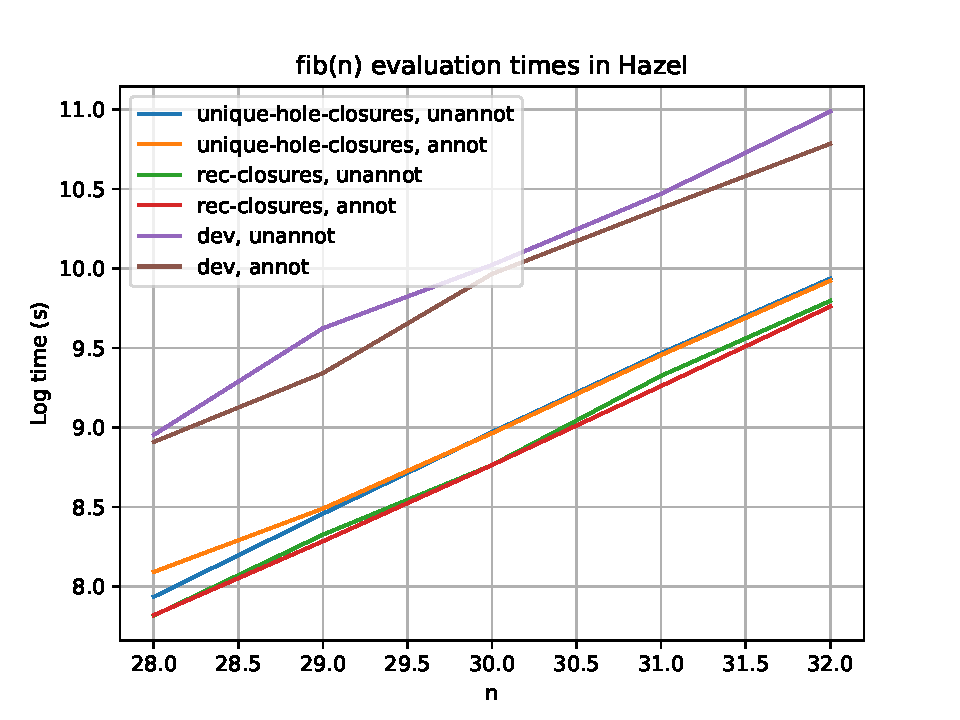
\includegraphics[width=10cm]{img/subst_evalenv_fib_perf.pdf}
%   \caption{Performance of the different models of evaluation}
%   \label{fig:perf_evaluation_models}
% \end{figure}

\begin{listing}
  \inputhminted{perf_fib}
  \caption{An evaluation-heavy Hazel program with no holes}
  \label{fig:perf-fib}
\end{listing}

\todo{also compare the performance of the above with the recursive data structures example}

\begin{listing}
  \inputhminted{perf_fib_more_bindings}
  \caption{An evaluation-heavy Hazel program with more variable bindings}
  \label{fig:perf-fib-more-bindings}
\end{listing}

\todo{note that there is now a "prologue" of some builtin functions: PI, int\_of\_float, float\_of\_int, and mod; these cause lookups to be slower because they take part of each lookup operation}

\begin{listing}
  \inputhminted{perf_fib_more_branches}
  \caption{An evaluation-heavy Hazel program with unused variable substitutions}
  \label{fig:perf-fib-more-branches}
\end{listing}

\section{Postprocessing performance}
\label{sec:evaluation-renumbering}

Consider the set of programs described by \Cref{fig:hole_renumbering_problem}.

\todo{describe this code blowup example}

\section{FAR performance}
\label{sec:evaluation-far}

\begin{singlespace}
  \begin{longtable}{p{20em} | p{7em} | p{7em}}
    \hline
    Program & Steps & Steps (w/ FAR) \\
    \hline\hline
    \inputhnfminted{far_hist_1} & & \\ \hline
    \inputhnfminted{far_hist_2} & & \\ \hline
    \inputhnfminted{far_hist_3} & & \\ \hline
    \inputhnfminted{far_hist_4} & & \\ \hline
    \inputhnfminted{far_hist_5} & & \\ \hline
    \inputhnfminted{far_hist_6} & & \\ \hline
    \inputhnfminted{far_hist_7} & & \\ \hline
    \inputhnfminted{far_hist_8} & & \\ \hline
    \inputhnfminted{far_hist_9} & & \\ \hline
    \inputhnfminted{far_hist_10} & & \\ \hline
    \hline
    \caption{A simple program edit history}
    \label{fig:far-program-history-simple}
  \end{longtable}
\end{singlespace}

\begin{singlespace}
  \begin{longtable}{p{20em} | p{7em} | p{7em}}
    \hline
    Program & Steps & Steps (w/ FAR) \\
    \hline\hline
    \inputhnfminted{far_fib_hist_1} & & \\ \hline
    \inputhnfminted{far_fib_hist_2} & & \\ \hline
    \inputhnfminted{far_fib_hist_3} & & \\ \hline
    \inputhnfminted{far_fib_hist_4} & & \\ \hline
    \inputhnfminted{far_fib_hist_5} & & \\ \hline
    \inputhnfminted{far_fib_hist_6} & & \\ \hline
    \inputhnfminted{far_fib_hist_7} & & \\ \hline
    \inputhnfminted{far_fib_hist_8} & & \\ \hline
    \hline
    \caption{A program edit history with an expensive computation}
    \label{fig:far-program-history-fib}
  \end{longtable}
\end{singlespace}

%%% Local Variables:
%%% mode: latex
%%% TeX-master: "main"
%%% End:
